\chapter{Applications: QML, Chemistry, Optimization and NISQ}\label{ch:applications}
\begin{center}\small\textit{From noisy 50-qubit chips to fault-tolerant dreams --- where quantum may actually help.}\end{center}

\section{Intuition: NISQ and Beyond}
We have $50$--$400$ qubit devices that are noisy and lack error correction. This is the NISQ era (Noisy Intermediate-Scale Quantum, Preskill 2018). They cannot run Shor on RSA-2048 (needs $\sim4000$ logical $\approx$ millions physical qubits). But they can try variational algorithms: a quantum circuit with tunable parameters prepares a state, a classical optimizer adjusts parameters to minimize a cost --- hybrid quantum-classical loops that tolerate some noise.

The big application bets are: quantum machine learning (QML), quantum chemistry/materials, and combinatorial optimization.

\section{Quantum Machine Learning}
Data $x$ is encoded into a quantum feature map $\lvert\phi(x)\rangle=U_{\phi}(x)\lvert0\rangle$. A parameterized circuit $W(\theta)$ processes it; measurement yields prediction. Training minimizes loss over $\theta$.

\begin{center}
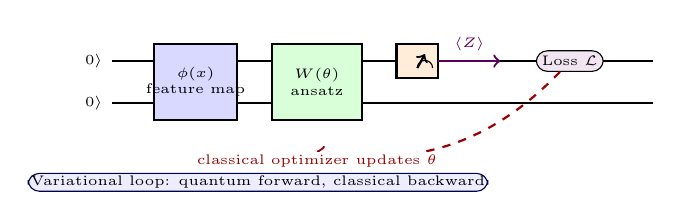
\begin{tikzpicture}[scale=0.88,font=\footnotesize]
  \draw[thick] (0,0.6)--(7.8,0.6);
  \draw[thick] (0,0)--(7.8,0);
  \node[left, font=\tiny] at (0,0.6) {$\lvert0\rangle$};
  \node[left, font=\tiny] at (0,0) {$\lvert0\rangle$};
  \draw[fill=blue!15, thick] (0.6,-0.25) rectangle (1.8,0.85) node[midway, align=center, font=\tiny] {$\phi(x)$\\feature map};
  \draw[fill=green!15, thick] (2.3,-0.25) rectangle (3.6,0.85) node[midway, align=center, font=\tiny] {$W(\theta)$\\ansatz};
  \draw[fill=orange!15, thick] (4.1,0.35) rectangle (4.7,0.85);
  \draw (4.4,0.5) arc (180:0:0.11); \draw[->, thick] (4.4,0.5)--(4.51,0.7);
  \draw[->, thick, violet!70!black] (4.7,0.6)--(5.6,0.6) node[midway, above, font=\tiny] {$\langle Z\rangle$};
  \node[draw, fill=violet!10, rounded corners, inner sep=2pt, font=\tiny] (loss) at (6.6,0.6) {Loss $\mathcal{L}$};
  \draw[->, thick, red!60!black, dashed] (loss) to[bend left=28] (2.95,-0.7) node[below, font=\tiny, fill=white, inner sep=1pt] {classical optimizer updates $\theta$};
  \node[font=\tiny, fill=blue!7, draw=blue!30!black, rounded corners, inner sep=1pt] at (2.1,-1.15) {Variational loop: quantum forward, classical backward};
\end{tikzpicture}
\end{center}

Quantum kernel methods use $K(x,x')=|\langle\phi(x)\vert\phi(x')\rangle|^2$ computed on hardware, then classical SVM. Advantage requires feature maps classically hard to simulate and datasets with quantum structure; for generic classical data, barren plateaus (gradients vanish exponentially in $n$) can kill training.

\begin{center}
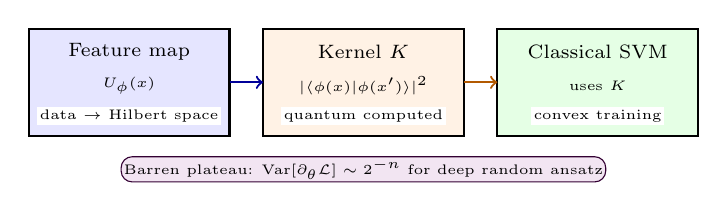
\begin{tikzpicture}[scale=0.85,font=\footnotesize]
  \fill[blue!10] (0,0) rectangle (3.0,1.6);
  \fill[orange!10] (3.5,0) rectangle (6.5,1.6);
  \fill[green!10] (7.0,0) rectangle (10.0,1.6);
  \draw[thick] (0,0) rectangle (3.0,1.6);
  \draw[thick] (3.5,0) rectangle (6.5,1.6);
  \draw[thick] (7.0,0) rectangle (10.0,1.6);
  \node[font=\scriptsize] at (1.5,1.25) {Feature map};
  \node[font=\tiny] at (1.5,0.75) {$U_\phi(x)$};
  \node[font=\tiny, fill=white, inner sep=1pt] at (1.5,0.3) {data $\to$ Hilbert space};
  \node[font=\scriptsize] at (5.0,1.25) {Kernel $K$};
  \node[font=\tiny] at (5.0,0.75) {$|\langle\phi(x)\vert\phi(x')\rangle|^2$};
  \node[font=\tiny, fill=white, inner sep=1pt] at (5.0,0.3) {quantum computed};
  \node[font=\scriptsize] at (8.5,1.25) {Classical SVM};
  \node[font=\tiny] at (8.5,0.75) {uses $K$};
  \node[font=\tiny, fill=white, inner sep=1pt] at (8.5,0.3) {convex training};
  \draw[->, thick, blue!60!black] (3.0,0.8)--(3.5,0.8);
  \draw[->, thick, orange!70!black] (6.5,0.8)--(7.0,0.8);
  \node[fill=violet!10, draw=violet!40!black, rounded corners, inner sep=1pt, font=\tiny] at (5.0,-0.5) {Barren plateau: $\mathrm{Var}[\partial_\theta\mathcal{L}]\sim2^{-n}$ for deep random ansatz};
\end{tikzpicture}
\end{center}

\section{Quantum Chemistry and VQE}
Molecular ground energy $E_0=\min_{\lvert\psi\rangle}\langle\psi|H|\psi\rangle$ where $H$ is the electronic Hamiltonian. VQE (variational quantum eigensolver) uses ansatz $\lvert\psi(\theta)\rangle$ and minimizes $\langle H\rangle$ measured termwise.

\begin{equation}
H=\sum_P h_P\,P,\quad P\in\{I,X,Y,Z\}^{\otimes n},\qquad
\langle H\rangle=\sum_P h_P\langle\psi(\theta)|P|\psi(\theta)\rangle.
\end{equation}
Each $\langle P\rangle$ is estimated by measuring that Pauli string. $FeMoco$, catalysts, and battery materials are target use cases; current VQE handles $10$--$20$ orbitals with noise mitigation.

\section{Optimization: QAOA}
For MaxCut, cost $C(z)=\sum_{(i,j)\in E}\tfrac12(1-z_iz_j)$, $z_i\in\{-1,1\}$. Map to Hamiltonian $H_C=\sum_{(i,j)}\tfrac12(1-Z_iZ_j)$. QAOA alternates

\begin{equation}
\lvert\gamma,\beta\rangle=e^{-i\beta_p H_M}e^{-i\gamma_p H_C}\cdots e^{-i\beta_1 H_M}e^{-i\gamma_1 H_C}\lvert+\rangle^{\otimes n},
\end{equation}
with mixer $H_M=\sum_i X_i$, then optimizes angles $\gamma,\beta$ classically. At depth $p\to\infty$, QAOA contains adiabatic evolution and is universal; at small $p$ it is a NISQ heuristic.

\begin{center}
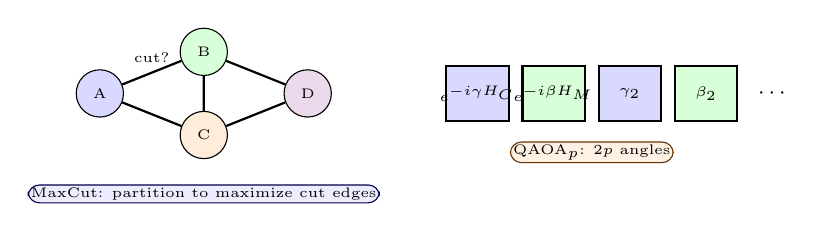
\begin{tikzpicture}[scale=0.88,font=\footnotesize]
  \node[draw, circle, fill=blue!15, minimum size=0.6cm, font=\tiny] (a) at (0,1.2) {A};
  \node[draw, circle, fill=green!15, minimum size=0.6cm, font=\tiny] (b) at (1.5,1.8) {B};
  \node[draw, circle, fill=orange!15, minimum size=0.6cm, font=\tiny] (c) at (1.5,0.6) {C};
  \node[draw, circle, fill=violet!15, minimum size=0.6cm, font=\tiny] (d) at (3.0,1.2) {D};
  \draw[thick] (a)--(b) node[midway, above, font=\tiny] {cut?};
  \draw[thick] (a)--(c); \draw[thick] (b)--(d); \draw[thick] (c)--(d); \draw[thick] (b)--(c);
  \node[font=\tiny, fill=blue!7, draw=blue!30!black, rounded corners, inner sep=1pt] at (1.5,-0.25) {MaxCut: partition to maximize cut edges};
  % QAOA block sequence
  \begin{scope}[shift={(5.0,1.2)}]
    \draw[fill=blue!15, thick] (0,-0.4) rectangle (0.9,0.4) node[midway, font=\tiny] {$e^{-i\gamma H_C}$};
    \draw[fill=green!15, thick] (1.1,-0.4) rectangle (2.0,0.4) node[midway, font=\tiny] {$e^{-i\beta H_M}$};
    \draw[fill=blue!15, thick] (2.2,-0.4) rectangle (3.1,0.4) node[midway, font=\tiny] {$\gamma_2$};
    \draw[fill=green!15, thick] (3.3,-0.4) rectangle (4.2,0.4) node[midway, font=\tiny] {$\beta_2$};
    \node at (4.7,0) {$\cdots$};
    \node[font=\tiny, fill=orange!10, draw=orange!40!black, rounded corners, inner sep=1pt] at (2.1,-0.85) {QAOA$_{p}$: $2p$ angles};
  \end{scope}
\end{tikzpicture}
\end{center}

\section{NISQ Limitations and Road Ahead}
NISQ devices lack correction: depth limited to $\sim10$--$100$ gates before noise dominates. Error mitigation (zero-noise extrapolation, Clifford data regression) stretches reach but not exponentially. Fault tolerance needs $10^3$--$10^4$ physical per logical qubit at $10^{-3}$ error. The path: better qubits $\to$ error mitigation $\to$ early correction $\to$ utility-scale advantage in chemistry and materials before breaking RSA.

\begin{center}
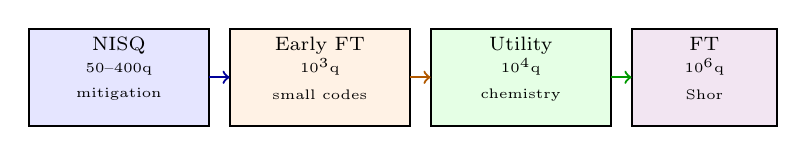
\begin{tikzpicture}[scale=0.88,font=\footnotesize]
  \fill[blue!10] (0,0) rectangle (2.6,1.4);
  \fill[orange!10] (2.9,0) rectangle (5.5,1.4);
  \fill[green!10] (5.8,0) rectangle (8.4,1.4);
  \fill[violet!10] (8.7,0) rectangle (10.8,1.4);
  \draw[thick] (0,0) rectangle (2.6,1.4);
  \draw[thick] (2.9,0) rectangle (5.5,1.4);
  \draw[thick] (5.8,0) rectangle (8.4,1.4);
  \draw[thick] (8.7,0) rectangle (10.8,1.4);
  \node[font=\scriptsize, align=center] at (1.3,1.0) {NISQ\\{\tiny 50--400q}};
  \node[font=\tiny] at (1.3,0.45) {mitigation};
  \node[font=\scriptsize, align=center] at (4.2,1.0) {Early FT\\{\tiny $10^3$q}};
  \node[font=\tiny] at (4.2,0.45) {small codes};
  \node[font=\scriptsize, align=center] at (7.1,1.0) {Utility\\{\tiny $10^4$q}};
  \node[font=\tiny] at (7.1,0.45) {chemistry};
  \node[font=\scriptsize, align=center] at (9.75,1.0) {FT\\{\tiny $10^6$q}};
  \node[font=\tiny] at (9.75,0.45) {Shor};
  \draw[->, thick, blue!60!black] (2.6,0.7)--(2.9,0.7);
  \draw[->, thick, orange!70!black] (5.5,0.7)--(5.8,0.7);
  \draw[->, thick, green!60!black] (8.4,0.7)--(8.7,0.7);
\end{tikzpicture}
\end{center}

\section{Python: VQE and QAOA Sketches}

\begin{lstlisting}[language=Python]
import numpy as np
from scipy.optimize import minimize

# VQE toy: H = Z0 Z1 + 0.5 X0 + 0.5 X1, 2 qubits
Z = np.array([[1,0],[0,-1]], complex)
X = np.array([[0,1],[1,0]], complex)
I = np.eye(2)
H = np.kron(Z,Z) + 0.5*np.kron(X,I) + 0.5*np.kron(I,X)
eigvals = np.linalg.eigvalsh(H)
print(f"Exact ground energy {eigvals[0]:.4f}")

def ansatz(theta):
    """Simple 2-qubit ansatz: Ry on each + CNOT."""
    ry = lambda t: np.array([[np.cos(t/2),-np.sin(t/2)],
                              [np.sin(t/2), np.cos(t/2)]])
    Ry0 = np.kron(ry(theta[0]), I)
    Ry1 = np.kron(I, ry(theta[1]))
    CNOT = np.array([[1,0,0,0],[0,1,0,0],[0,0,0,1],[0,0,1,0]], complex)
    psi0 = np.array([1,0,0,0], complex)
    return CNOT @ Ry1 @ Ry0 @ psi0

def vqe_cost(theta):
    psi = ansatz(theta)
    return np.real(psi.conj() @ H @ psi)

res = minimize(vqe_cost, x0=[0.5, -0.3], method='COBYLA')
print(f"VQE energy {res.fun:.4f} at {res.x}")
\end{lstlisting}

\begin{lstlisting}[language=Python]
# QAOA MaxCut p=1 on 4-node cycle
import numpy as np
from scipy.optimize import minimize

# 4-cycle edges
edges = [(0,1),(1,2),(2,3),(3,0)]
n = 4; N = 2**n

def cost_hamiltonian():
    Hc = np.zeros((N,N), complex)
    for i,j in edges:
        for z in range(N):
            bits = [(z>>k)&1 for k in range(n)]
            zi, zj = 1-2*bits[i], 1-2*bits[j]  # +1/-1
            Hc[z,z] += 0.5*(1 - zi*zj)
    return Hc

Hc = cost_hamiltonian()
# p=1 QAOA expectation
def qaoa_expect(params):
    gamma, beta = params
    # |+>^n
    plus = np.ones(N, complex)/np.sqrt(N)
    # e^{-i gamma Hc} diagonal, e^{-i beta sum X} = product Ry-like
    diag = np.exp(-1j*gamma*np.diag(Hc))
    psi = diag * plus
    # Mixer: apply Rx(2beta) on each qubit via brute force
    # Simplified: approximate by exponentiating sum X (small n)
    X = np.array([[0,1],[1,0]], complex)
    Xm = sum(np.kron(np.kron(np.eye(2**i), X), np.eye(2**(n-1-i)))
             for i in range(n))
    Um = np.linalg.matrix_power(np.eye(N) -1j*beta*Xm, 1)  # first order
    # Use exact expm for accuracy
    from scipy.linalg import expm
    Um = expm(-1j*beta*Xm)
    psi = Um @ psi
    return -np.real(psi.conj() @ Hc @ psi)  # negative for minimize

res = minimize(qaoa_expect, x0=[0.5, 0.5], method='COBYLA')
print(f"QAOA p=1 best cut {-res.fun:.3f} (opt=4) at gamma,beta={res.x}")
\end{lstlisting}

\section{Exercises}
\begin{exercise}
For VQE with $H=Z\otimes Z$, what is the single-qubit $R_y$ ansatz minimum? Show entanglement (CNOT) is not needed for this $H$ but is for $H=X\otimes X+Y\otimes Y$.
\end{exercise}
\begin{exercise}
MaxCut on a triangle (3 nodes, 3 edges): enumerate all cuts, find optimum, then simulate QAOA $p=1$ and plot $\langle H_C\rangle$ over $\gamma,\beta\in[0,\pi]$.
\end{exercise}
\begin{exercise}
Explain barren plateaus: for a random $n$-qubit ansatz, show $\mathrm{Var}[\partial_k\mathcal{L}]$ decays exponentially in $n$ and discuss how local cost functions and shallow depth mitigate it.
\end{exercise}
\begin{exercise}
Compare quantum kernel $K_{ij}=|\langle\phi(x_i)\vert\phi(x_j)\rangle|^2$ with classical RBF. When would you expect quantum advantage? Propose a dataset built from discrete-log structure.
\end{exercise}
\begin{exercise}
Estimate physical qubits needed for Shor on RSA-2048: assume distance $d=27$ surface code, $2d^2$ physical per logical, $\sim4000$ logical qubits. What error budget does this imply?
\end{exercise}
